% !TeX spellcheck = en_GB

ToC
Modelling the TSP
\begin{enumerate}
	\item Ops perspective
	\item Smoothing the hard constraint, the pragmatic perspective
\end{enumerate}
Tryna solve the TSP
\begin{enumerate}
	\item Local search
	\begin{itemize}
		\item \texttt{swap}
		\item \texttt{swap-rev} or \texttt{reverse}
	\end{itemize}
	\item Simulated annealing
	\item Multi-start
\end{enumerate}
Results
\begin{itemize}
	\item Convergence analysis and other diagnostics
	\item Energy view using multi-start
	\item What's next? Simulated tempering (SA with reheating), genetics algorithms
\end{itemize}
References
\begin{itemize}
	\item Collega di Pisa? Quelli che trovavo su Medium? Paper trovati per caso?
\end{itemize}

% ***************************************************** %
\section{Modelling the travelling salesman problem}\label{sc:tsp}
% ***************************************************** %

Given an undirected (weighted) and complete graph $G=(V,E)$, where the set of all nodes $\abs{V}=N$ and the set of all edges $\set{i,j}$ is $\abs{E}=N(N-1)/2$ and their relative weight $c_{ij}>0$. an Hamiltonian cycle is a cycle which touches every node in $V$ once and only once, an Hamiltonian cycle might not exist.

% TODO: add all possible edges
We consider the two following layouts with all possible edges\par\smallskip
\begin{center}
	\begin{minipage}{0.4\textwidth}
		\newcount\mycount
		\begin{tikzpicture}[transform shape]
			\draw [help lines,pink] (-2.5,-2.5) grid (2.5,2.5);% \node[circle,draw,fill=red] at (0,0) {};
			
			\def \n {8}
			\def \radius {2}

			\foreach \i in {1,2,...,\n}{%
				\node[graphnode] (\i) at ({-360/\n * (1 - \i)}:\radius) {\i};
			}
%			\foreach \number in {1,...,15}{
%				\mycount=\number
%				\advance\mycount by 1
%				\foreach \numbera in {\the\mycount,...,16}{
%					\path ($16-\number$) edge[->,bend right=3] ($16-\numbera$) edge[<-,bend
%					left=3] ($16-\numbera$);
%				}
%			}
%			\foreach \i in {1,2,...,\n-1}{%
%				\mycount=\i
%				\advance\mycount by 1
%				\foreach \j in {\the\mycount,...,\n}{%
%%					\draw[->] ($\n-\i$) to ($\n-\j$);
%					\path ()
%				}
%			}
		\end{tikzpicture}%\captionof{figure}{Circular layout}
	\end{minipage}\quad
	\begin{minipage}{0.4\textwidth}
		\begin{tikzpicture}
			\draw [help lines,pink] (-2.5,-2.5) grid (2.5,2.5);% \node[circle,draw,fill=red] at (0,0) {};
			
			\foreach \i/\j in {(1.09582419,-1.48754547)/1, (-0.24448624,-0.19845625)/2, (1.43439168,-0.5168079)/3, (0.78947212,1.70705996)/4, (-1.62329061,0.57546048)/5, (1.90248941,1.29104645)/6, (1.04455881,-0.2263432)/7, (1.14425722,-1.09104511)/8}{%
				\node[graphnode] at \i {\j};
			}
		\end{tikzpicture}%\captionof{figure}{Random layout}
	\end{minipage}
\end{center}
on the left, a circular graph, for which we know that the optimal solution is a circular path; on the right each node is in a random position, so we don't know exactly the optimal solution.

We constraint the Hamiltonian cycle to start with the first node 1, so the total number of possible cycles reduces to $(N-1)!$.


% ***************************************************** %
\subsection{The optimization perspective}
% ***************************************************** %

The Travelling Salesman Problem (TSP) consists in finding the \emph{shortest Hamiltonian cycle}. The feasible set $F$ is the set of all Hamiltonian cycles in $G$ and the objective function $c(P)$ is the length of the Hamiltonian cycle $P$.

We make use of a logical variable for each edge
\[
x_{ij}=
\begin{cases}
	1 & \text{if $i\rightarrow j$} \\
	0 & \text{otherwise}
\end{cases}
\]
hence the objective function si the sum of all costs associated with the edges in the cycle. This is the binary constraint on variables.

Since a feasible solution is a cycle, we must impose the constraint that each node has one incoming and one outgoing edge\par
\begin{center}
	\begin{tikzpicture}
		\draw [help lines,pink] (-2.5,-1.25) grid (2.5,1.25);

		\node[graphnode,fill=white,font=\footnotesize] (h) at (-1.2,-0.8) {$h$};
		\node[graphnode,font=\normalsize] (i) at (0,0.5) {$i$};
		\node[graphnode,fill=white,font=\footnotesize] (k) at (1.5,0.1) {$k$};
		
		\draw[->,thick] (h) -- (i); \draw[->,thick] (i) -- (k);
	\end{tikzpicture}
\end{center}
that is the \emph{cycle covering} constraint.

Using only this constraint can result in a solution with sub-tours, so we add a constraint for connecting all possible sub-tours\par\medskip
\begin{center}
	\begin{minipage}{0.32\textwidth}
		\begin{tikzpicture}
			\tikzset{help lines/.append style=pink}
			\draw [help lines] (-0.5,-1.5) grid (4.5,1.5);% \node[circle,draw,fill=red] at (0,0) {};
			
			%% nodes
			\node[graphnode] (1) at (0,1) {1}; \node[graphnode] (2) at (2,1) {2}; \node[graphnode] (3) at (4,1) {3};
			\node[graphnode] (4) at (1,0) {4};
			\node[graphnode] (5) at (0,-1) {5}; \node[graphnode] (6) at (2,-1) {6}; \node[graphnode] (7) at (4,-1) {7};
			
			%% edges
			\draw[thick] (1) -- (4) -- (6) -- (5) -- (1);
			\draw[thick] (2) -- (3) -- (7) -- (2);
			%	\foreach \i in {0,1,...,6}{%
				%		\foreach \j in {0,1,...,6} {%
					%			\draw (\i) -- (\j);
					%		}
				%	}
		\end{tikzpicture}
	\end{minipage}%
	\quad%
	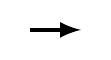
\begin{tikzpicture}
		\draw[-latex,ultra thick] (-0.4,0) -- (0.25,0);
	\end{tikzpicture}%
	\quad%
	\begin{minipage}{0.31\textwidth}
		\begin{tikzpicture}
			\draw (0,0) ellipse (0.8 and 1.1); \node[right] at (0.5,0.9) {$V\setminus S$};
			\draw (-2,-1) ellipse (0.6 and 0.7); \node[left] at (-2.5,-0.5) {$S$};
			
			\node[graphnode] (i) at (-1.9,-1.15) {$i$};
			\node[graphnode] (j) at (0.2,0) {$j$};
			
			\draw[->] (i) -- (j);
		\end{tikzpicture}
	\end{minipage}%\quad\quad%$\Leftarrow$\quad
\end{center}
from a subset $S$ there must be at least an edge to the complementary set $V\setminus S$, the \emph{connection} constraint, that is the \emph{hard} constraint.

The resulting optimization problem will be
\begin{equation}\label{eq:tsp-prob}
	\begin{aligned}
		\min\quad & c(P)=\sum_{\set{i,j}\in E}c_{ij}x_{ij} \\
		& \sum_{\set{i,j}\in E}x_{ij}=2 \\
		& \sum_{i\in S,j\notin S}x_{ij}\geq1\quad\emptyset\subset S\subset V \\
		& x_{ij}\in\set{0,1}
	\end{aligned}
\end{equation}

In practice, for simplicity, the cost for each edge is the distance between the two cities, so we use the distance matrix $D\in\R^{N\times N}$
\[
D=(d_{ij})=
\begin{pmatrix} 
	0 & d_{12} & d_{13} & \cdots & d_{1N} \\
	d_{21} & 0 & d_{23} & \cdots & d_{2N} \\
	d_{31} & d_{32} & 0 & \cdots & d_{3N} \\
	\vdots & \vdots & \vdots & \ddots & \vdots \\
	d_{N1} & d_{N2} & d_{N3} & \cdots & 0
\end{pmatrix}
\]
that is a symmetric matrix, whether an edge is in the cycle or not, the variables $x_{ij}$ become the elements of the adjacency matrix $A$ of the same shape of $D$. The objective function will be $c(P)=A\odot D$ that we call $f$ for simplicity; the cycle covering constraint becomes the sum over rows and columns of $A$ that must be equal to $2N$.

%% problem informal description
%Given a list of cities of size $N$ and their relative distances in a matrix , what is the shortest path that visits each city exactly once and returns to the origin city?

%% problem mathematical description

%\begin{align}\label{eq:tsp}
%\min & A\odot D \\
% & \boldsymbol{1}^TA\boldsymbol{1}=1 \\
% & \boldsymbol{1}^TA_Q\boldsymbol{1}\leq\abs{Q}-1
%\end{align}

%\begin{equation}
%\begin{align*}%{lll}
%\min_{a_{ij}} & \sum_{i=1}^N\sum_{\substack{j=1\\i\neq j}}^Nd_{ij}a_{ij} \\
% & \sum_{i=1,i\neq j}^Na_{ij}=1 & i=1,\dots,N \\
% & \sum_{j=1,i\neq j}^Na_{ij}=1 & j=1,\dots,N \\
% & \sum_{\substack{i\in Q}}\sum_{j\in Q,i\neq j}a_{ij}\leq\abs{Q}-1 & \forall Q\subset\set{1,\dots,N},\abs{Q}\geq2
%\end{align*}
%\end{equation}

% TODO: consider summarizing with a table
What kind of algorithms?
\begin{itemize}
	\item heuristics
	\item meta-heuristics
\end{itemize}

Which algorithms?
\begin{itemize}
	\item Brute-force
	\begin{itemize}
		\item Swap indices
		\item Swap indices and reverse middle indices
		\item Check all permutations
	\end{itemize}
	\item Meta-heuristics
	\begin{itemize}
		\item Multi-start (GRASP)
		\item Simulated Annealing (SA)
	\end{itemize}
\end{itemize}

%\begin{figure}
%\centering
%\begin{tikzpicture} % add adjacency matrix?
%	\tikzset{help lines/.append style=pink}
%	\draw [help lines] (-1,-1) grid (4,2);
%
%	%% nodes
%	\node[graphnode] (0) at (0,0) {0};
%	\node[graphnode] (1) at (1,1.5) {1};
%	\node[graphnode] (2) at (3,1) {2};
%	\node[graphnode] (3) at (2,-0.5) {3};
%
%	%% edges
%	\draw[-stealth] (0) to node[left,font=\small] {$d_{01}$} (1);
%	\draw[-stealth] (1) to node[above,font=\small] {$d_{12}$} (2);
%	\draw[-stealth] (2) to node[right,font=\small] {$d_{23}$} (3);
%	\draw[-stealth] (3) to node[below,font=\small] {$d_{30}$} (0);
%\end{tikzpicture}
%\caption{Example circular disposition}
%\label{fig:tsp-graph}
%\end{figure}


% ***************************************************** %
\subsection{Smoothing the hard constraint}
% ***************************************************** %

% TODO: how to satisfy the hard constraint within the algorithms





\cleardoublepage
% ***************************************************** %
\subsection{Local search}\label{subsc:local-search}
% ***************************************************** %

The idea behind this class of algorithms is simple: given a feasible solution, there might be some other similar feasible solutions with lower objective function value. So the idea is to optimize the objective function by exploring the neighborhood of the current point in the solution space.

The local search starts with a feasible solution randomly drawn in the feasible set. A generation mechanism is then successively applied in order to find a better solution, in terms of the objective function value, by exploring the neighborhood of the current solution.

The algorithm ends when no improvement can be found, and the current solution is considered as the approximate solution of the optimization problem.

%\begin{algorithm}\caption{Local search framework}
%\KwIn{$x^0$}
%$k\gets 0$\;
%\While{$\sigma(x^k)\neq x^k$}{%
	%	$\sigma(x^k)\gets\argmin_yc(y)\mid y\in I(x^k)$\;
	%	$x^{k+1}\gets\sigma(x^k)$\;
	%}
%\end{algorithm}

\begin{algorithm}\caption{Local search framework}\label{alg:local-search}
	\KwIn{$f$, $D$, $x^0$}
	$x^\ast\gets x^0$\;
	$k\gets 0$\;
	\While{stopping criterion not satisfied}{%
		Generate a feasible solution $\bar{x}$ s.t. $\bar{x}\in I(x^\ast)$\;
		\If{$f(\bar{x})<f(x^\ast)$}{%
			$x^\ast\gets\bar{x}$\;  % this implies to fully explore each I(x^\ast)
		}
		$k\gets k+1$\;
	}
	\KwOut{$x^\ast$}
\end{algorithm}

If the current solution falls in a subdomain over which the objective function is convex, the algorithm remains trapped in this subdomain. In order to avoid being trapped in local minimum, it is then necessary to define a process likely to accept current feasible solutions that momentarily reduce the performance (objective function value) of the current solution.


\begin{algorithm}\caption{Multi-start framework}\label{alg:multi-start}
	\KwIn{$f$, $D$}
	$x^\ast$ s.t. $f(x^\ast)=\infty$\;
	\For{$b=1,2,\dots,B$}{%
		Generate a starting feasible solution $x^0$\;
		Perform a local search (algorithm~\ref{alg:local-search}) starting from $x^0$ to obtain $x^b$\;
		\If{$f(x^b)<f(x^\ast)$}{%
			$x^\ast\gets x^b$\;
		}
	}
	\KwOut{$x^\ast$}
\end{algorithm}



% ***************************************************** %
\subsection{Simulated annealing}
% ***************************************************** %

\begin{defs}[Metropolis acceptance criterion]
	Let $(S,f)$ be an instantiation of a combinatorial minimization problem, and $i,j$ two points of the state space. The acceptance criterion for accepting solution $j$ from the current solution $i$ si given by the following probability:
	\[
	\mathbb{P}(\text{accept $j$})=
	\begin{cases}
		1 & \text{if $f(j)<f(i)$} \\
		\exp(-(f(j)-f(i))/c) & \text{otherwise}
	\end{cases}
	\]
	where $c$ is the control parameter.
\end{defs}

\begin{defs}[Transition]
	A transition represents the replacement of the current solution $i$ by a neighboring solution. This operation is carried out in two stages: generation and acceptance.
\end{defs}



\begin{algorithm}\caption{Simulated Annealing (SA)}\label{alg:sim-ann}
	\KwIn{$f$, $D$, $x^0$, $T_0$, $\alpha$, $L_k$}
	%Perform few SA iterations repeatedly to obtain $T_0$ with high acceptance rate\;
	$x^\ast\gets x^0$\;
	$k\gets0$\;
	\While{stopping criterion not satisfied}{%
		$x^k\gets x^\ast$\;
		\For{$i=1,2,\dots,L_k$}{%
			Generate a feasible solution $\bar{x}$ s.t. $\bar{x}\in I(x^\ast)$\;
			\If{$f(\bar{x})<f(x^\ast)$}{%
				$x^\ast\gets\bar{x}$\tcp*[l]{down-hill, new best solution}
			}
			
			\uIf{$f(\bar{x})<f(x^k)$}{%
				$x^k\gets\bar{x}$\tcp*[l]{down-hill note that $f(x^k)\geq f(x^\ast)$}
			}
			\Else{%
				Generate a random number $r\sim U(0,1)$\;
				$\Delta E\gets f(\bar{x})-f(x^k)$\tcp*[l]{energy gap}
				\If{$r<\exp(-\Delta E/T_k)$}{%
					$x^k\gets\bar{x}$\tcp*[l]{up-hill, lower quality solution accepted}
				}
			}
		}
		$T_{k+1}\gets\alpha T_k$\;
		$k\gets k+1$\;
	}
	\KwOut{$x^\ast$}
\end{algorithm}





































